\section{Bazar Blot Game}\label{ModelDescription}
\lhead{AI algorithms used for the game}
\subsection{Hill Climbing Algorithm for Bidding}
\hspace{\parindent}You can find a provided template for the Belote AI model.
The general environment consists of a player and 3 AIs; let’s call them \textit{Left
AI}, \textit{Right AI} and \textit{Top AI}. The first stage of the game is the implementation of
the bidding part, where each player should bid a number for the hand they received
and try to negotiate with their partner. We decided to use the Hill-Climbing Algorithm by
using a manual and mildly complicated heuristic for each player pair and each
possible suit available to bid on (\textit{Spades, Hearts, Diamonds, Clubs, No-Trumps}). The
Algorithm will count the heuristic value for each suit, compare it to the opponents’
bid, and take into account the partner’s previous bid. The main operation will include
giving a weight to the higher cost cards (Aces and Tens for the Suit “Aces”, Jacks and
Nines for the rest), add the partner’s bid to the corresponding suit, find the maximum
among the 5 possibilities, and compare it to the opponents’ bid.
\par Scenario


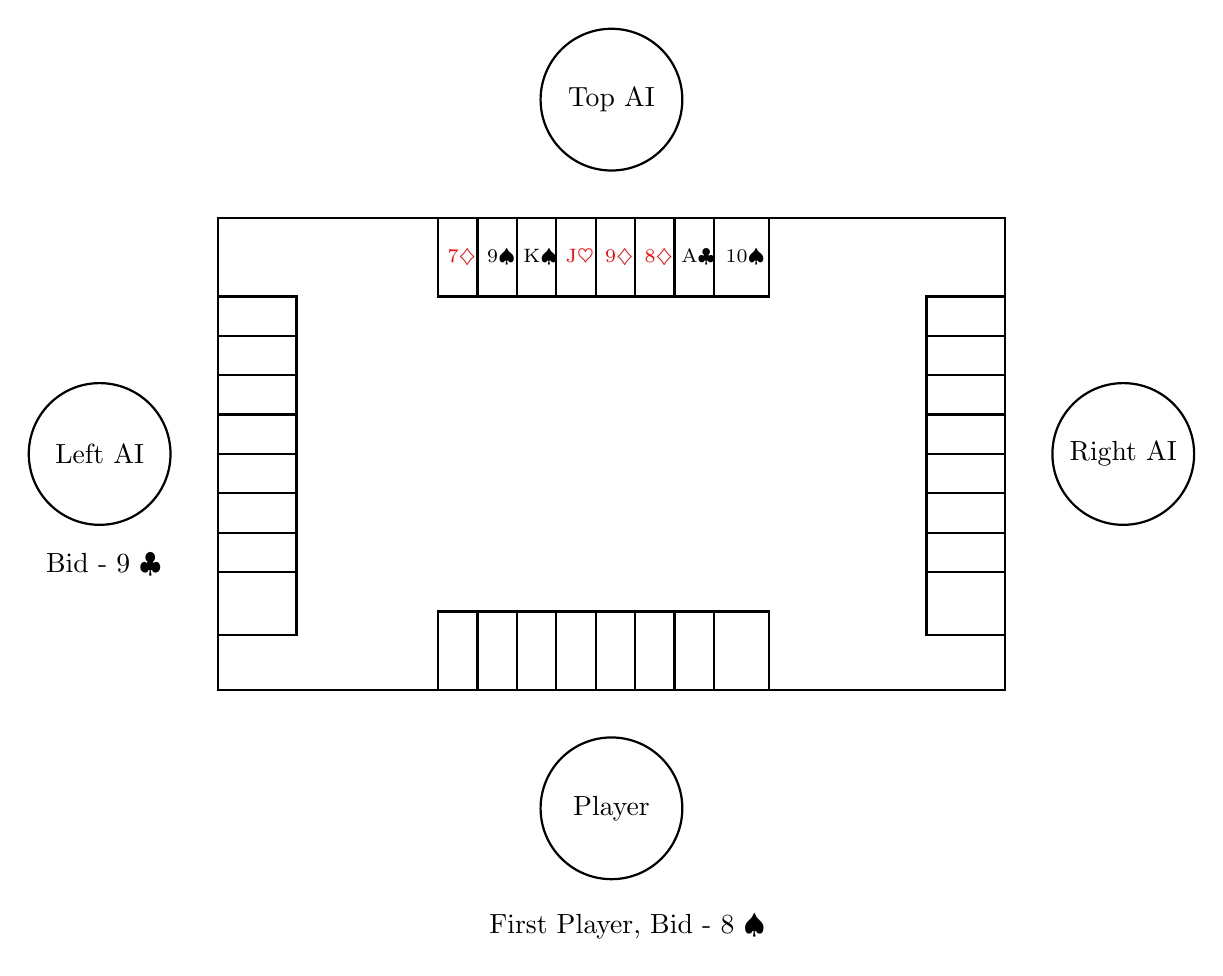
\begin{tikzpicture}

\draw[thick] (0,0) rectangle (10,6);  % Rectangle table dimensions

\foreach \i in {0,1,2,3,4,5,6,7}
    \draw[thick, draw=black, fill=white] (1, 5-\i*0.5) rectangle (0, 5-\i*0.5-0.8);
\foreach \i in {0,1,2,3,4,5,6,7}
    \draw[thick, draw=black, fill=white] (10, 5-\i*0.5) rectangle (9, 5-\i*0.5-0.8);
\foreach \i in {0,1,2,3,4,5,6,7}
    \draw[thick, draw=black, fill=white] (2.8 + \i*0.5, 6) rectangle (3.5 + \i*0.5, 5);
\foreach \i in {0,1,2,3,4,5,6,7}
    \draw[thick, draw=black, fill=white] (2.8 + \i*0.5, 0) rectangle (3.5 + \i*0.5, 1);

\draw[thick] (-1.5, 3) circle(0.9);
% Right side chair
\draw[thick] (11.5, 3) circle(0.9);
% Top side chair
\draw[thick] (5, 7.5) circle(0.9);
% Bottom side chair
\draw[thick] (5, -1.5) circle(0.9);

\node at (-1.5, 3) {Left AI};
\node at (-1.45, 1.6) {Bid - 9 $\clubsuit$};
\node at (11.5, 3) {Right AI};
\node at (5, 7.5) {Top AI};
\node at (5, -1.5) {Player};
\node at (5.2, -3) {First Player, Bid - 8 $\spadesuit$};

\node at (3.1, 5.5) {\scriptsize \textcolor{red}{7$\diamondsuit$}};
\node at (3.6, 5.5) {\scriptsize \textcolor{black}{9$\spadesuit$}};
\node at (4.1, 5.5) {\scriptsize \textcolor{black}{K$\spadesuit$}};
\node at (4.6, 5.5) {\scriptsize \textcolor{red}{J$\heartsuit$}};
\node at (5.1, 5.5) {\scriptsize \textcolor{red}{9$\diamondsuit$}};
\node at (5.6, 5.5) {\scriptsize \textcolor{red}{8$\diamondsuit$}};
\node at (6.1, 5.5) {\scriptsize \textcolor{black}{A$\clubsuit$}};
\node at (6.7, 5.5) {\scriptsize \textcolor{black}{10$\spadesuit$}};

\end{tikzpicture} \pagebreak

If at the start of the game you recalled 8 Spades, and the opponent (Left AI), raised the bid to 9 Clubs,
your partner’s algorithm will look into the hand; say it has these cards (7$\diamondsuit$, 9$\spadesuit$, King$\spadesuit$,
Jack$\heartsuit$, 9$\diamondsuit$, 8$\diamondsuit$, Ace$\clubsuit$, 10$\spadesuit$). The heuristic value for each of the suits would be;

\begin{itemize}
    \item Diamonds:  14 = 0 (8$\diamondsuit$) + 14 (9$\diamondsuit$) + 0 (7$\diamondsuit$),
    \item Spades: 32 = 4 (King$\spadesuit$) + 14 (9$\spadesuit$) + 10 (1$\spadesuit$0) + 1/2 x 8 (Partner’s Bid),
    \item Hearts: 20 (Jack $\heartsuit$),
    \item Clubs: 6.5 = 11 (Ace$\clubsuit$) - 1/2 x 9  (Opponents’ Bid),
    \item No Trumps: 25 = 4 (King$\spadesuit$) + 19 (Ace$\clubsuit$) + 2 (Jack$\heartsuit$)
\end{itemize}

Here it is obvious that the AI
is going to call its partner’s bid (Spades, as it has the highest heuristic value), the question is: How much? There is another logic
imported that would decide if there is a need for the AI to increase the bid by 1, 2 or
more, and the main logic is going to contain the possible additional points from special
combinations (like Tierce giving 2 points), it will also include the bade suit heuristic
value divided 20 (as each 10 heuristic equals to 1 point, and divided with another 2 for emergency)
and rounded and will be added to the point
count, in this case we will have a Tierce (7$\diamondsuit$, 8$\diamondsuit$, 9$\diamondsuit$) and heuristic difference of 32/20
= 1.6, rounded to 2. The point count would include adding 4 points to the partner’s bid,
hence the algorithm will return 12 Spades. There are going to be extra conditions for
the actions Coinchee, Cabot, etc.)


\subsection{Minimax Algorithm for the Playing part}
\hspace{\parindent} Up to the Second phase of the game, which is the playing process.
In this case, we will use
the Stochastic Minimax Algorithm, which will work for each trick (each player making one
move after which it is calculated which side gets the cards). At the beginning of the
game, there will be a set trump, which will prioritize the moves of the players,
especially if their bid won. If your bid did not win, and the play starts with you,
the minimax algorithm will prioritize using high value non-trump cards, however, the
algorithm should check, if the opponents will either have a higher value card from the
same suit, or no cards of the corresponding suit. As an example, Let’s imagine that the
play starts with the AI, the bid belongs to opponents, and it is set to be 11$\spadesuit$.
The bot has 1 trump card (Q$\spadesuit$), 3$\clubsuit$, 2$\diamondsuit$, and 10$\heartsuit$. The highest
non-trump card is 10$\heartsuit$. The Minimax algorithm, will check all the branches with
possible combinations of 8 cards for the opponent, and return possibilities for cases
when the bot team wins, or when the opponents win. In this case, it would be 2/3 chance
for the opponents to have the Ace$\heartsuit$, 1/3 chance for the partner to have Ace$\heartsuit$. We add
to this the probability that one of the opponents does not have any Hearts hence they
will use the trump. If we approximate, we will calculate the chances of not having any
of the remaining 6 hearts out of 24 (p=0.25) and calculate the probability using Binomial
Distribution on 8 cases with 0 successes, returning 0.1 for each player (chance of not
having a Hearts card). For at least one player to not have any hearts card, we will get
19% chance for at least one of the opponents not having any Hearts. As a result we would
get the union of the probabilities and get the 86% chance of losing the H10 by playing it.
Hence the Stochastic Minimax will play
the card with 86% chance. Instead of using Binomial Distribution, the algorithm will
check the possible outcomes of the play, and calculate the proportion, when the H10 is
lost to opponents, and hence get the probability of success. This process would be done
for each prioritized card to play, until the best option is picked (Highest success rate).
If the bot is prone to lose the card nonetheless, then it is chosen to be the least value
having card on the hand.